\documentclass[reqno,11pt]{amsart}
\usepackage{amsmath, amssymb, amsthm}
\usepackage{url}
\usepackage{moreverb}
\usepackage{algorithm}
\usepackage{algorithmicx}
\usepackage{algpseudocode}
\usepackage{pgfplots}
\usepackage{xspace}
\theoremstyle{plain}
\newtheorem{prop}{Proposition}[section]
\theoremstyle{definition}
\newtheorem{defi}[prop]{Definition}
\newtheorem{nota}[prop]{Notation}
\newtheorem{exam}[prop]{Example}
\newtheorem{lem}[prop]{Lemma}
\newtheorem{fact}[prop]{Fact}

\title{Exploring the tree of numerical semigroups}
\author{Jean Fromentin and  Florent Hivert}

\newcommand{\gr}[1]{{\color{gray} #1}}
%\newcommand{\card}{\#}
\newcommand{\ie}{\emph{i.e.}}
\newcommand{\Cilk}{\texttt{Cilk}\xspace}
\newcommand{\CilkP}{\texttt{Cilk++}\xspace}
\newcommand{\CPP}{\texttt{C++}\xspace}
\newcommand{\kkp}{{k+1}}
\newcommand{\gen}[1]{\left<#1\right>}
\renewcommand{\leq}{\leqslant}
\renewcommand{\geq}{\geqslant}
\newcommand{\MMX}{\texttt{MMX}\xspace}
\newcommand{\SIMD}{\texttt{SIMD}\xspace}
\newcommand{\SSE}{\texttt{SSE}\xspace}
\newcommand{\SSEV}{\texttt{SSE4.1}\xspace}
\newcommand{\NN}{\mathbb{N}}
\renewcommand{\tt}[1]{\texttt{#1}}
\newcommand{\sgnode}[1]{{\bf \left<#1\right>}}
\renewcommand{\ie}{\emph{i.e}}
\DeclareMathOperator{\Irr}{Irr}
\DeclareMathOperator{\App}{App}
\DeclareMathOperator{\card}{card}
\newcommand{\Jean}[1]{{\color{blue}#1}}
\newcommand{\Florent}[1]{{\color{green}#1}}
\newcommand{\Delete}[1]{}
\newcommand{\REM}[1]{\marginpar{\small #1}}
\newcommand{\TODO}[1]{\marginpar{\small To do: #1}}

\begin{document}

\begin{abstract}
In this paper we describe an algorithm visiting all the numerical semigroups up to a given genus using a new representation of numerical semigroups. 
\end{abstract}

\maketitle

\section{Introduction}

A \emph{numerical semigroup} $S$ is a subset of $\NN$ containing $0$, close under addition and of finite complement in $\NN$.  
For example the set 
\begin{equation}
\label{E:NSG}
S_E=\{0,3,6,7,9,10\}\cup[12,+\infty[
\end{equation}
is a numerical semigroup.
The \emph{genus} of a numerical semigroup $S$, denoted by~$g(S)$, is the cardinality of $\NN\setminus S$.
 For example the genus of $S_E$ is $6$,  the cardinality of $\{1,2,4,5,8,11\}$

For a given positive integer $g$, the number of numerical semigroups of genus $g$ is finite and is denoted by $n_g$. 
In  J.A. Sloane's \emph{on-line encyclopedia of integer}~\cite{OEIS} we find the values of $n_g$ for $g\leq 52$. 
These values have been obtain by M. Bras-Amor\'os (view \cite{BrasAmoros2008} for more details for $g\leq 50)$. 
On his home page~\cite{Delgado}, M. Delgado  gives the value of $n_{55}$ without specifying the values of $n_{53}$ and~$n_{54}$. 

M.~Bras-Amor\'os used a depth first search exploration of the tree of numerical semigroups $\mathcal{T}$ up to a given genus.
This tree was introduced by J.C.~Rosales and al. in \cite{Rosales} and it is the subject of the Section~\ref{S:Tree}.
Starting with all the numerical semigroups of genus $49$ she obtained the number of numerical semigroups of genus $50$ in $18$ days on a pentium D runing at $3$GHz. 
In the package~\tt{NumericalSgs} \cite{NumericalSgps} of \tt{GAP} \cite{GAP}, M. Delgado together with P.A.~Garcia-Sanchez and J. Morais used the same method of exploration.


\Jean{Here we describe a new algorithm for the exploration of the tree of numerical semigroup $\mathcal{T}$ and achieve the computation of $n_g$ for $g\leq 67$. 
The cornerstone of our method is a new combinatorial representation of numerical semigroup that is well suited for exploration of the tree~$\mathcal{T}$ and allow code optimization essentially based on use of vectorial instructions and parallelization.}



The paper is divided as follows.
In Section~\ref{S:Tree} we describe the tree of numerical semigroups and give bounds for some parameters attached to a numerical semigroup.
\Jean{The decription of our new representation of numerical semigroup is done in the third section.}
\Delete{In Section~\ref{S:Tree} we describe a new representation of numerical semigrouos that is well suited to the construction of the tree.}
In Section~\ref{S:Algo} we describe an algorithm based on the representation given in Section~\ref{S:DecNumber} and give its complexity. 
Section~\ref{S:Opti} is more technical, and is devoted to the optimisation of the algorithm introduced in Section~\ref{S:Algo}.

\section{The tree of numerical semigroups}
\label{S:Tree}

We start this section with definitions and properties of numerical semigroups that will be used in the sequel.
For a more complete introduction, the reader can usefully consults the book \emph{Numerical Semigroups} of J.C.~Rosales and P.A.~Garc\'ia-S\'anchez \cite{BookNS} or the book \emph{The Diophantine Frobenius Problem} of J.L.~Ram\'irez~Alfons\'in \cite{BookDFP}.

\begin{defi}
Let $S$ be a numerical semigroup. We define 

$i)$ $m(S)=\min(S\setminus\{0\})$, the \emph{multiplicity} of $S$;

$ii)$ $g(S)=\card(\NN\setminus S)$, the \emph{genus} of $S$;

$iii)$ $c(S)=1+\max(\NN\setminus S)$, the \emph{conductor} of $S$ for $S$ different from $\NN$. By convention, the conductor of $\NN$ is $0$. 
\end{defi}

By definition a numerical semigroup is an infinite object. 
We need a finite description of such a semigroup. 
That is the role of generating sets.


\begin{defi}
A subset $X=\{x_1<x_2<...<x_n\}$ of a semigroup is a \emph{generating set} of $S$ if every element of $S$ can be expressed as a sum of elements in $X$. 
In this case we write $S=\left<x_1,...,x_n\right>$.
\end{defi}

If we reconsider the numerical semigroup of \eqref{E:NSG}, we obtain
\begin{equation}
\label{E:GNSG}
S_E=\{0,3,6,7,9,10\}\cup[12,+\infty[=\left<3,7\right>
\end{equation}


A non-zero element $x$ of a numerical semigroup $S$ is said to be \emph{irreducible} if it cannot be expressed as a sum of two non-zeros elements of $S$.  
We denote by $\Irr(S)$ the set of all irreducible elements of $S$.

\begin{lem}[Lemma 2.3, Chap. I, \cite{BookNS}]
Let $S$ be a numerical semigroup. The set $\Irr(S)$ is the minimal generating set of $S$ relatively to the inclusion ordering.
\end{lem} 


%\begin{proof}
%Assume for a contradiction, that there exists an integer  $x$ in $S$ than cannot be decomposed as a sum of irreducible elements. 
%We may assume that $x$ is  minimal with this property. 
%As  $x$ cannot be irreducible, there exist $y$ and $z$ in~$S\setminus\{0\}$ satisfying $x=y+z$. 
%Since we have $y<x$ and $z<x$, the integers $y$ and $z$ can be expressed as a sum of irreducible elements of $S$ and so $x=y+z$ is a sum of irreducible elements, in contradiction to hypothesis. 
%
%As irreducible elements of $S$ cannot be decomposed as the sum of two non-zeros integers in $S$, they must occur in each generating set of $S$.
%\end{proof}


%Let $S$ be a numericla semigroup. As $m(S)$ lies in $S$ the irreducible elements are include in
%\[
%\App(S)=\{x\in S \, |\, x-m(S)\not\in S\}
%\]
%The set $\App(S)$ is the so-called Ap\'ery set relativey to the element $m(S)$.
%
%\begin{lem}[Lemma 2.4, Chap. I, \cite{BookNS}]
%Let $S$ be a numerical semigroup. The Apéry set $\App(S)$ is finite of cardinality $m(S)$.
%\end{lem}
%
%The following result is a direct consequence of the previous Lemma and the Inclusion of $\Irr(S)$ in $m(S)$.
%
%\begin{prop}
%\label{P:Res}
%A numerical semigroup has at most $m(S)$ irreducible elements.
%\end{prop}

The differents parameters we have defined on a numerical semigroup, statisfy the following relations.

\begin{prop}
\label{P:Res}
Let $S$ be a numerical semigroup. We have

$i)$  $x\in \Irr(S)$ implies $x\leq c(S)+m(S)-1$;

$ii)$ $m(S)\leq g(S)+1$;

$iii)$ $c(S)\leq 2 g(S)$.
\end{prop}

\begin{proof}
$i)$ Let $x$ ba a positive integer satisfying $x \geq c(S)+m(S)$. 
As the integers $x$ and $x-m(S)$ are greater than $c(S)$, they belong to $S$.
Since $x$ equals $(x-m(S))+m(S)$ with $x-m(S)\not=0$ and $m(S)\not=0$, it could not be irreducible.

$ii)$ The set $\NN\setminus{S}$ of cardinality $g(S)$ contains $\{1,..,m(S)-1\}$ and so the relation $m(S)\leq g(S)+1$ holds.

$iii)$ Let $x$ be an element of $S\cap[0,c(S)-1]$. 
The integer $y=c(S)-1-x$ lies in $[0,c(S)-1]$. 
Moreover $y$ is not in $S$, for otherwise  we write $c(S)-1=y+x$ where $x,y$ are elements of $S$ implying $c(S)-1\in S$. 
In contradiction with the definition of conductor. 
Thus we define an involution 
\[
\begin{array}{rcl}
\psi:[0,c(S)-1]&\to&[0,c(S)-1]\\
x&\mapsto&c(S)-1-x
\end{array}
\]
that send $S\cap[0,c(S)-1]$ into $[0,c(S)-1]\setminus S$ which is  of cardinality $g(S)$. 
Let us denote by $k$ the cardinality  of $S\cap[0,c(S)-1]$. 
Since $\psi$ is injective we must have $k\leq g(S)$. 
From the relation 
\[
[0,c(S)[=S\cap[0,c(S)[\sqcup[0,c(S)[\setminus S
\]
 we obtain $c(S)=k+g(S)$ and so $c(S)\leq 2 g(S)$.
\end{proof}

A consequence of Proposition~ \ref{P:Res}~$i)$ is that $\Irr(S)$ is finite and its cardinality is at most $c(S)+m(S)-1$.
More precisely, using Ap\'ery set, we can prove that  the cardinality of $\Irr(S)$ is at most $m(S)$. See Section 2 of Chapter I of~\cite{BookNS} for more details.

We now explain the construction of the tree of numerical semigroups.
Let~$S$ be a numerical semigroup. The set $T=S\cup\{c(S)-1\}$ is also a numerical  semigroup and its genus is $g(S)-1$. 
As  $[c(S)-1,+\infty[$ is included in $T$ we have $c(T)\leq c(S)-1$. 
Therefore every semigroup $S$ of genus $g$ can be obtained from a semigroup $T$ of genus $g-1$ by removing an element of~$T$ greater than or equal to $c(T)$.

\begin{prop}
\label{P:Sx}
Let $S$ be a numerical semigroup and $x$ an element of $S$. The set~$S^x=S\setminus\{x\}$ is a numerical semigroup if and only if $x$ is irreducible in $S$.
\end{prop}


\begin{proof}
If $x$ is not irreducible in  $S$, then there exist $a$ and $b$ in $S\setminus{0}$ such that $x=a+b$. 
Since $a\not=0$ and $b\not=0$ hold, the integers  $a$ and $b$ belong to $S\setminus\{x\}$. 
Since $x=a+b$ and $x\not\in S^x$, it follows that  $S^x$ is not stable under addition. 

Conversely, assume that $x$ is irreducible in  $S$. 
As $0$ is never irreducible, the set~$S^x$ contains~$0$. 
Let $a$ and $b$ be two integers belonging to $S^x$. 
The set~$S$ is stable under addition, hence $a+b$ lies in $S$. 
As $S$ is equal to $S^x\cup\{x\}$, the integer $a+b$ also lies in $S^x$ except if it is equal to $x$. 
The latter is impossible since $a$ and $b$ are different from $x$ and $x$ is irreducible.
\end{proof}

Proposition~\ref{P:Sx} implies that every semigroup $T$ of genus $g$ can be obtained from a semigroup $S$ by removing a generator $x$ of $S$ that is greater than $c(S)$.
Hence relations~$T=S^x=S\setminus\{x\}$ hold.

We construct the tree of numerical semigroups, denoted by $\mathcal{T}$ as follows. 
The root of the tree is the unique semigroup of genus $0$, \ie, $\left<1\right>$ that is equal to $\NN$. 
If~$S$ is a semigroup in the tree,  the sons of $S$ are exactly the semigroup~$S^x$ where $x$ belongs to $\Irr(S)\cap[c(s),+\infty[$. 
By convention, when depicting the tree, the numerical semigroup $S^x$ is in the left of $S^y$ if $x$ is smaller than~$y$. 
With this construction, a semigroup $S$ has depth $g$ in $\mathcal{T}$ if and only if its genus is~$g$, see Figure~\ref{F:Tree}.
We denote by $\mathcal{T}_{\leq g}$ the subtree of $\mathcal{T}$ resticted to all semigroup of genus $\leq g$.


 \begin{figure}[hf!]
 % \[
 % \pstree[,nodesep=3pt]{\sgnode{1}}{
 % 	\pstree[nodesep=3pt]{\sgnode{2,3} \tlput1}{
 % 		\pstree[treesep=4pt,nodesep=2pt]{\sgnode{3,4,5} \tlput2}{
 % 			\pstree[treesep=3pt,nodesep=3pt]{\sgnode{4,5,6,7} \tlput3}{
 % 				\pstree{\sgnode{5,6,7,8,9} \tlput4}{}
 % 				\pstree{\sgnode{\gr 4,6,7,9} \tlput5}{}
 % 				\pstree{\sgnode{\gr 4,\gr 5,7} \trput6}{}
 % 				\pstree{\sgnode{\gr 4,\gr 5,\gr 6} \trput7}{}
 % 			}
 % 			\pstree[treesep=3pt,nodesep=3pt]{\sgnode{\gr 3,5,7} \tlput4}{
 % 				\pstree{\sgnode{\gr 3,7,8} \tlput 5}{}
 % 				\pstree{\sgnode{\gr 3,\gr 5} \trput 7}{}
 % 			}
 % 			\pstree[treesep=10pt]{\sgnode{\gr 3,\gr 4} \trput5}{\Tn \Tn \Tn}
 % 		}
 % 		\pstree[nodesep=3pt]{~\hspace{-5em}\sgnode{\gr2,5} \trput3}{
 % 			\pstree[nodesep=3pt]{\sgnode{\gr2,7} \trput5}{
 % 				\pstree[nodesep=3pt]{\sgnode{\gr2,9} \trput7}{}
 % 			}
 % 		}
 % 	}
 % }
 % \vspace{-5em}
 % \]

\[
\begin{tikzpicture}[level distance=2cm, inner sep=2mm,
  level/.style={sibling distance=1.55cm},
%  edge from parent/.style={draw}
  ]
    \node {$\sgnode{1}$}
    child {node {$\sgnode{2,3}$}
      child [sibling distance=4.5cm] {node {$\sgnode{3,4,5}$}
        child {node {$\sgnode{4,5,6,7}$}
          child [sibling distance=2cm]{node {$\sgnode{5,6,7,8,9}$}  edge from parent node [left] {4}}
          child [sibling distance=1.9cm]{node {$\sgnode{\gr 4,6,7,9}$}  edge from parent node [left] {5}}
          child {node {$\sgnode{\gr 4,\gr 5,7}$}  edge from parent node [right] {6}}
          child {node {$\sgnode{\gr 4,\gr 5,\gr 6}$}  edge from parent node [right] {7}}
          edge from parent node [left] {3}
        }
        child{{} edge from parent[draw=none]}
        child{{} edge from parent[draw=none]}
        child {node {$\sgnode{\gr 3,5,7}$}
          child {node {$\sgnode{\gr 3,7,8}$} edge from parent node [left] {5}}
          child {node {$\sgnode{\gr 3,\gr 5}$} edge from parent node [right] {7}}
          edge from parent node [left] {4}
        }
        child {node {$\sgnode{\gr 3,\gr 4}$}
          edge from parent node [right] {5}
        }
        edge from parent node [left] {2}
      }
      child [sibling distance=4.5cm] {node {$\sgnode{\gr2,5}$}
        child {node {$\sgnode{\gr2,7}$}
          child {node {$\sgnode{\gr2,9}$}
            edge from parent node [right] {7}
          }
          edge from parent node [right] {5}
        }
        edge from parent node [right] {3}
      }
      edge from parent node [left] {1}
    }
    ;
  \end{tikzpicture}
  \]
\caption{The first four layers of the tree $\mathcal{T}$ of numerical semigroups, corresponding to $\mathcal{T}_{\leq 4}$. A generator of a semigroup is in gray if it is not in $[c(S),+\infty[$. An edge between a semigroup $S$ and its son $S'$ is labelled by  $x$ is $S'$ is obtained from $S$ by removing~$x$, that is $S'=S^x$.}
\label{F:Tree}
\end{figure}

As the reader can check, the main difficulty to characterize the son of a semigroup is to determine its irreducible elements.
 In \cite{NumericalSgps}, the semigroup are given by their Ap\'ery set and then the difficulty is to describe the Ap\'ery set of $S_x$  from this of $S$. 
 This approach is elegant but not sufficiently \emph{basic} for our optimisations.



\section{Decomposition number}
\label{S:DecNumber}

The aim of this section is to describe a new representation of numerical semigroups.
which is well suited to an efficient exploration of the tree~$\mathcal{T}$ of numerical semigroups. 

\begin{defi}
Let $S$ be a numerical semigroup.
For every $x$ of $\NN$  we set
\[
D_S(x)=\{y \in S\ |\ x-y\in S\ \text{and}\ 2y\leq x\}
\]
and $d_S(x)=\card D_S(x)$.
We called $d_S(x)$ the $S$-\emph{decomposition number} of~$x$.
The application $d_S:\NN\to\NN$ is the $S$-\emph{decomposition numbers function}.
\end{defi}

Assume that $y$ is an element of $D_S(x)$.
By very definition of $D_S(x)$, the integer~$z=x-y$ also belongs to $S$. 
Then $x$ can be decomposed as $x=y+z$ with $y$ and $z$ in~$S$. 
Moreover the condition $2y\leq x$ implies $y\leq z$. 
In other words if we define~$D'_S(x)$ to be the set of all $(y,z)\in S\times S$ with $x=y+z$ and $y\leq z$ then~$D_S(x)$ is the image of $D'_S(x)$ under the projection on the first coordinate.
 Hence~$D_S(x)$ describes how~$x$ can be decomposed as sums of two elements of $S$.
 This is we decide to call $d_S(x)$ the $S$-decomposition number of $x$.

\begin{exam}
Reconsider the semigroup $S_E$ given at \eqref{E:NSG}.
The integer $14$ admits three decompositions as sums of two elements of $S$, namely $14=0+14$, $14=3+11$ and $14=7+7$. 
Thus the set $D_{S_E}(14)$ is equal to $\{0,3,7\}$ and $d_{S_E}$ equals $3$.
\end{exam}


\begin{lem}
\label{L:RepN}
For every numerical semigroup $S$ and every integer $x\in \NN$,  we have $d_S(x)\leq 1+\left\lfloor \dfrac{x}2\right\rfloor$ and the equality holds for $S=\NN$.
\end{lem}

\begin{proof}
As the set $D_S(x)$ is included in $\{0,...,\left\lfloor\frac x2\right\rfloor\}$, the relation $d_S(x)\leq 1+\left\lfloor \frac{x}2\right\rfloor$ holds.
For $S=\NN$ we have the equality for $D_S(x)$ and so for $d_S(x)$.
\end{proof}


\begin{prop}
\label{P:Dandd}
Let $S$ be a numerical semigroup and $x\in\NN\setminus\{0\}$.  We have:

 $i)$ $x$ lies in $S$ if and only if $d_S(x)>0$.

 $ii)$ $x$ is in $\Irr(S)$ if and only if $d_S(x)=1$.
\end{prop}

\begin{proof}
We start with $i)$. If $x$ is an element of $S$ then $x$ equals $0+x$. 
The relation~$2\times 0\leq x$ and $0\in S$ imply that $D_S(x)$ contains $0$, and so $d_S(x)>0$ holds.
Conversely, the relation  $d_S(x)>0$  implies that $D_S(x)$ is non-empty. 
Let $y$ be an element of~$D_S(x)$. 
As $y$ and $x-y$ belong to  $S$, by definition, the integer $x=(x-y)+y$ is in $S$  (since $S$ is stable by addition).

Let us show $ii)$. 
Assume $x$ is irreducible in $S$.
There cannot exist $y$ and $z$ in~$(S\setminus\{0\})^2$ such that $x=y+z$. 
The only possible decomposition of $x$ as a sum of two elements of $S$ is $x=0+x$. 
Hence, the set $D_S(x)$ is equal to~$\{0\}$ and we have $d_S(x)=1$. 
Conversely, let $x$ such that $d_S(x)$ is $1$. 
By  $i)$ the  integer $x$ must be in $S$. 
As $x=0+x$ is always a decomposition of $x$ as a sum of two elements in $S$, we obtain $D_S(x)=\{0\}$.
If there exist $y$ and $z$ in $S$ such that $y\leq z$ and $x=y+z$ hold then $y$ lies in $D_S(x)$. 
This implies $y=0$ and $z=x$. 
Hence $x$ is irreducible in~$S$.
\end{proof}

We note  that $0$ is never irreducible despite the fact $d_S(0)$ is $1$ for all numerical semigroup $S$.

We now explain how to compute the $S$-decomposition numbers function of a numerical semigroup  from this of its father.

\begin{prop}
Let $S$ be a numerical semigroup and $x$ be an irreducible element of $S$. 
Then for all $y\in \NN\setminus\{0\}$ we have
\[
d_{S^x}(y)=\begin{cases}
d_S(y)-1&\text{if $y\geq x$ and $d_S(y-x)>0$,}\\
d_S(y) &\text{otherwise.}
\end{cases}
\] 
\end{prop}


\begin{proof}
Let $y$ be in $\NN\setminus\{0\}$. We have 
\[
D_{S^x}(y)=\{z \in S^x\ |\ y-z\in S^x\ \text{and}\  2z\leq y\}.
\]
We construct three sets as follow:
\begin{align*}
E&=\{z\in S^x\ |\ y-z=x\ \text{and}\ 2z\leq y\}\\
F&=\begin{cases}
\{x\}&\text{if $y-x\in S$ and $2x\leq y$},\\
\emptyset&\text{otherwise}.
\end{cases}
\end{align*}
We have the relation $D_{S}(y)=D_{S^x}(y)\sqcup E\sqcup F$ and so $d_S(y)$ is equal to $d_{S^x}(y)+\card(E)+\card(F)$.
and $D_{S^x}(y)$ is a subset of $D_S(y)$. We start by determining $E$. 
The relation $y-z=x$ implies $z=y-x$ and $2z\leq y$ becomes $y\leq 2x$. Thus we obtain
\[
E=\begin{cases}
\{y-x\}&\text{if $y-x\in S^x$ and $y\leq 2x$}\\
\emptyset&\text{otherwise}
\end{cases}
\] 
The relation $y-x\in S^x$ together with $y\leq2x$ is equivalent to $y-x\in S$ together with $y<2x$.
Therefore we obtain
\[
E=\begin{cases}
\{y-x\}&\text{if $y-x\in S$ and $y< 2x$}\\
\emptyset&\text{otherwise}
\end{cases}
\] 
Assume $y-x$ lies in $S$.  If $y<2x$ holds, we have $E=\{y-x\}$ and $F=\emptyset$. Otherwise, we obtain $E=\emptyset$ and $F=\{x\}$. 
Then if $y-x\in S$ holds, we have $\card(E)+\card(F)=1$ and so $d_{S}(y)$ is equal to $d_{S^x}(y)+1$.
If $y-x$ not belong to $S$, then $E$ and $F$ are empty implying $d_{S}(y)=d_{S^x}(y)$. As the condition $y-x\in S$ is equivalent to $y\geq x$ together with $d_S(y-x)>0$ by Proposition~\ref{P:Dandd} the result holds.
\end{proof}

\section{A new algorithm}
\label{S:Algo}
We can easily explore the tree of numerical semigroups up to a genus $G$ using
a depth first search algorithm (see Algorithm~\ref{A:ExpRec}). This approach does not seem to
have been used before.  In particular, M. Bras-Amor\'os and M. Delgado use
instead a breadth first search exploration.  The main advantage in our
approach is the small memory needs.  The cost to pay is that, if we want to
explore the tree deeper, we must restart from the root.
\begin{algorithm}
\caption{Recursive Depth first search exploration of the tree of numerical semigroups}\label{A:ExpRec}
\begin{algorithmic}[1]
\Procedure{ExploreRec}{\tt{S}, \tt{G}}
	\If{$g(\tt{S})< \tt{G}$}
		\For{\tt{x} from $c(\tt{S})$ to $c(\tt{S})+m(\tt{S})$}
			\If{$\tt{x}\in \Irr(\tt{S})$}
				\State \Call{ExploreRec}{$\tt{S}^\tt{x}, \tt{G}$}
			\EndIf
		\EndFor
	\EndIf
\EndProcedure
\State \Call{ExploreRec}{$\NN, \tt{G}$}
\end{algorithmic}
\end{algorithm}

Equivalently, we can use an iterative version which uses a stack (see Algorithm~\ref{A:Exp}).
\begin{algorithm}
\caption{Iterative Depth first search exploration of the tree of numerical semigroups}\label{A:Exp}
\begin{algorithmic}[1]
\Procedure{Explore}{\tt{G}}
\State Stack \tt{stack} \Comment{the empty stack}
\State $\tt{S} \gets\left<1\right>$
\While{stack is not empty} 
	\State $\tt{S} \gets \tt{stack.top()}$
	\State \tt{stack.pop()}
	\If{$g(\tt{S})< \tt{G}$}
		\For{\tt{x} from $c(\tt{S})$ to $c(\tt{S})+m(\tt{S})$}
			\If{$\tt{x}\in \Irr(\tt{S})$}
				\State $\tt{S.push}(\tt{S}^\tt{x})$
			\EndIf
		\EndFor
	\EndIf
\EndWhile
\EndProcedure
\end{algorithmic}
\end{algorithm}

In Algorithm~\ref{A:ExpRec} we do not specify how to compute $c(S)$, $g(S)$ and $m(S)$  from $S$ neither how to test if an integer is irreducible. 
It also miss  the characterisation of $S^x$ from $S$.
These items depend heavily of the representation of $S$.
Our choice is to use the $S$-decomposition numbers function. 
The first task is to use a finite set of such numbers to characterise the whole semigroup.

\begin{prop}
\label{P:delta}
Let $G$ be an integer and $S$ be a numerical semigroup of genus $g\leq G$.
Then $S$ is entirely described by $\delta_S=(d_S(0),...,d_S(3\,G))$. More precisely we can obtain $c(S), g(S), m(S)$ and $\Irr(S)$ from $\delta_S$.
\end{prop} 

\begin{proof}
By Proposition~\ref{P:Res} $iii)$ we have $c(S)\leq 2g(S)$ and so the $S$-decomposition number of $c(S)$ occurs in $\delta_S$.
Since $c(S)$ is equal to $\max(\NN\setminus S)$, Proposition~\ref{P:delta} implies 
\[
c(S)=1+\max\{i\in[0,...,3G],\ d_S(i)=0\}.
\]
As all elements of $\NN\setminus S$ are smaller than $c(S)$, their $S$-decomposition numbers are in $\delta_S$ and we obtain
\[
g(S)=\card\{i\in[0,..,3G],\ d_S(i)=0\}.
\]
By Proposition~\ref{P:Res} $ii)$, the relation $m(S)\leq g(S)+1$ holds. 
This implies that the $S$-decomposition number of $m(S)$ appears in $\delta_S$ : 
\[
m(S)=\min\{i\in[0,...,3G],\ d_S(i)>0\}.
\]
Since, by Proposition~\ref{P:Res} $i)$,  all irreducible elements are smaller than $c(S)+m(S)-1$, which is itself smaller than $3G$ the relations $ii)$ and $iii)$ of Proposition~\ref{P:Res} give
\[
\Irr(S)=\{i\in[0,...,3G],\ d_S(i)=1\}.
\]
\end{proof}

Even though it is quite simple, the computation of $c(S),m(S)$ and $g(S)$ from $\delta_S$ has a non negligible cost.
We represent a numerical semigroup $S$ of genus $g\leq G$ by $(c(S),g(S),c(S),\delta_S)$. 
In an algorithmic context, if the variable \texttt{S} stands for a numerical semigroup  we use:

-- \tt{S.c}, \tt{S.g} and \tt{S.m} for the integers $c(S)$, $g(S)$ and $m(S)$;

-- \tt{S.d[i]} for the integer $d_S(i)$.

For example the following Algorithm initializes a representation of the semigroup $\NN$ ready for an exploration up to genus $G$.

\begin{algorithm}
\caption{Return the root of $\mathcal{T}$ for an exploration up to genus \tt{G}}\label{A:Root}
\begin{algorithmic}
\Function{Root}{\tt{G}}
\State \tt{R.c} $\gets$ 1 \Comment{\tt{R} stands for $\NN$}
\State \tt{R.g} $\gets$ 0
\State \tt{R.m} $\gets$ 1 
\For{\tt{x} from $1$ to $3\,\tt{G}$}
	\State\tt{R.d[x]}$\gets1+\left\lfloor\frac{\tt{x}}2\right\rfloor$
\EndFor
\State{\textbf{return} \tt{R}}
\EndFunction
\end{algorithmic}
\end{algorithm}

We can now describe an algorithm that returns the representation of the semigroup $S^x$ from that of the semigroup $S$ where $x$ is an irreducible element of $S$ greater than $c(S)$.

\begin{algorithm}
\caption{Returns the son $S_x$ of $S$ with $x\in\Irr(S)\cap[c(S),c(S)+m(S)[$.}\label{A:Son}
\begin{algorithmic}[1]
\Function{Son}{\tt{S},\tt{x},\tt{G}}
\State \tt{T.c} $\gets$ $\tt{x}+1$ \Comment{\tt{T}  stands for $\tt{S}_x$}
\State \tt{T.g} $\gets$ $\tt{S.g}+1$
\If{$\tt{x}>\tt{S.m}$}
	\State \tt{T.M} $\gets$ \tt{S.m}
\Else
	\State \tt{T.M} $\gets$ $\tt{S.m}+1$
\EndIf
\State\tt{T.d} $\gets$ \tt{S.d}
\For{\tt{y} from \tt{x} to $3\,\tt{G}$}
	\If{$\tt{S.d}[\tt{y}-\tt{x}]>0$}
		\State $\tt{T.d}[\tt{y}]\gets\tt{T.d}[\tt{y}]-1$
	\EndIf
\EndFor
\State{\textbf{return} \tt{T}}
\EndFunction
\end{algorithmic}
\end{algorithm}

\begin{prop}
\label{P:Son}
Running on $(S,x,G)$ with $g(S)\leq G$, $x\in \Irr(S)$ and~$x\leq c(S)$, Algorithm~\ref{A:Son} returns the numerical semigroup $S_x$ in time $O(\log(G)\times G)$.
\end{prop}

\begin{proof}
By construction $S^x$ is the semigroup $S\setminus\{x\}$.
Thus the genus $S^x$ is $g(S)+1$, see Line~\tt{1}.
Every integer of $I=[x+1,+\infty[$ lies in $S$ since $x$ is greater than $c(S)$, so the interval $I$ is included in $S^x$.
As $x$ does not belong to $S$, the conductor of $S^x$ is $x+1$, see Line \tt{2}.
For the multiplicity of $S^x$ we have two cases. 
First, if $x>m(S)$ holds  then $m(S)$ is also in $S^x$ and so $m(S^x)$ is equal to $m(S)$.
Assume now $x=m(S)$. 
The relation $x(S)\geq c(S)$ and the characterisation of~$m(S)$ implies $x=m(S)=c(S)$.
Thus $S^x$ contains $m(S)+1$ which is $m(S^x)$.
The initialisation of $m(S^x)$ is done by Lines \tt{4} to \tt{8}. 
The correctness of the computation of $\delta_{S^x}$ (see Proposition~\ref{P:delta}) done from Line \tt{9} to Line \tt{15} is a direct consequence of~Proposition~\ref{P:Dandd}. 

Let us now prove the complexity statement. 
Since by relations $ii)$ and $iii)$ of Proposition~\ref{P:Res} we have $x\leq 3G$ together with $m(S)\leq G+1$, each line from \tt{2} to \tt{8} is done in time $O(\log(G))$.
The \textbf{for} loop needs $O(G)$ steps and each step is done in time $O(\log(G))$. 
Summarizing, these results give that the algorithm runs in time $O(\log(G)\times G)$.
\end{proof}

\begin{algorithm}
\caption{Returns an array containing the value of $n_g$ for $g\leq G$}\label{A:Count}
\begin{algorithmic}[1]
\Function{Count}{\tt{G}}
\State \tt{n} $\gets [0,...,0]$ \Comment $\tt{n[g]}$ stands for $n_g$ and is initialised to $0$
\State Stack \tt{stack} \Comment{the empty stack}
\State $\tt{S} \gets \textsc{Root}(\tt{G})$
\While{stack is not empty} 
	\State $\tt{S} \gets \tt{stack.top()}$
	\State \tt{stack.pop()}
	\State $\tt{n[S.g]}\gets\tt{n[S.g]}+1$
	\If{$\tt{S.g}< \tt{G}$}
		\For{\tt{x} from $\tt{S.c}$ to $\tt{S.c}+\tt{S.m}$}
			\If{$\tt{S.d[x]\,=\,1}$}
				\State $\tt{S.push}(\textsc{Son}(\tt{S},\tt{x},\tt{G}))$
			\EndIf
		\EndFor
	\EndIf
\EndWhile
\State{\textbf{return} \tt{n}}
\EndFunction
\end{algorithmic}
\end{algorithm}

\begin{prop}
Running on $G\in\NN$, Algorithm \textsc{Count} returns the array~$[n_0,...,n_G]$ in time
\[
O\left(\log(G)\times G \times \sum_{g=0}^G n_g\right)
\]
and its space complexity is $O(\log(G)\times G^3)$.
\end{prop}

\begin{proof}
The correctness of the algorithm is a consequence of Proposition~\ref{P:Son} and of the description of the tree~$\mathcal{T}$ of numerical semigroups.

For the time complexity, let us remark that Algorithm~\textsc{Son} is called for every semigroup of the tree $\mathcal{T}^{\leq G}$ (the restriction of $\mathcal{T}$ to semigroup of genus $\leq G$). 
Since there are exactly $N=\sum_{g=0}^G n_g$ such semigroups, the time complexity of \textsc{Son} established in Proposition~\ref{P:Son} guarantees that the running time of \textsc{Count} is in~$O(\log(G)\times G\times N)$, as stated.

Let us now prove the space complexity statement.
For  this we need to describe the stack through  the run of the algorithm.
Since the stack is filled  with a depth first search algorithm, it has two properties.
The first one is that reading the stack from the bottom to the top, the genus of  semigroup increases.  
The second one is that, for all $g\in[0,G]$, every semigroup of genus $g$ in the stack has the same father.
As the number of sons of a  semigroup $S$ is the number of $S$-irreducible elements in $[c(S),c(S)+m(S)-1]$,  a semigroup $S$ has at most $m(S)$ sons. 
By~Proposition~\ref{P:Res} $ii)$, this implies that a semigroup of genus $g$ as at most $g+1$ sons.
Therefore the stack contains at most $g+1$ semigroup of genus $g+1$ for $g\leq G$. 
So the size of the stack is bounded~by 
\[
S=\sum_{g=0}^Gg=\frac{G(G+1)}2
\]
A semigroup is represented by a quadruple $(c(S),g(S),m(S),\delta_S)$. 
By relations $ii)$ and $iii)$ of Proposition~\ref{P:Res}, we have $c\leq 2g(S)$ and $m\leq g(S)+1$. 
As $g(S)\leq G$ holds, the integers~$c$, $g$  and $m$ of the representation of $S$ require a memory space in $O(\log(G))$. 
The size of~$\delta_S=(d_S(0),...,d_S(3G))$ is exactly~$3G+1$. 
Each entry of $\delta_S$ is the $S$-decomposition number of an integer smaller than $3G$ and hence
requires $\log(G)$ bytes of memory space.
Therefore the space complexity of $\delta_S$ is in~$O(\log(G)\times G)$, which implies that the space complexity of the \textsc{Count} algorithm is
\[
O(\log(G)\times G\times S)= O(\log(G)\times G^3).
\]
\end{proof}

\section{Technical optimizations and results}

\label{S:Opti}

Though there are asymptotically faster algorithms than the one presented here,
thank to careful optimizations, we were able to compute $n_g$ for much larger
genus than before. This is due to the fact that our algorithm is particularly
well suited for the current processor architecture. In particular, it allows
to use parallelism at various scale (parallel branch exploration,
vectorization)...

To get the greatest speed from modern processor, we used several optimization
tricks, which we will elaborate in the following section:

\REM{C'est un peu moche c'est gros points, non? Des tirets peut etre.}
\begin{itemize}
\item Vectorization (\MMX, \SSE instructions sets) and careful memory alignment. 
\item Shared memory multi-core computing using \CilkP for low level
  enumerating tree branching;
\item Partially derecursived algorithm using a stack;
\item Avoiding all dynamic allocation during the computation: everything is
  computed ``in place'';
\item Avoiding all unnecessary copy (the cost of the \textsc{Son} algorithm is
  roughly the same as copying) !
\item Aggressive loop unrolling: the main loop is unrolled by hand using some
  kind of Duff's device.
\item Carefull choice of data type (\verb|uint_fast8_t| for decomposition
  number, vs \verb|uint_fast64_t| for all indexes).
\end{itemize}

\subsection{Vectorization}

Assume for example that we want to construct the tree~$\mathcal{T}^{\leq 100}$
of all numerical semigroup of genus smaller than $100$.  In this case, the
representation of numerical semigroup given in Section~\ref{S:DecNumber} uses
decomposition numbers of integers smaller than~$300$.  By Lemma~\ref{L:RepN},
such a decomposition number is smaller than $151$ and requires~$1$ byte of
memory.  Thus at each \textbf{for} step of Algorithm~\textsc{Son}, the CPU
actually works on $1$ byte. However current CPUs usually work on $8$ bytes and
even on $16$~bytes using vector extensions. \REM{Peut etre rajouter qqchose sur l'AVX; en fait on devrait pouvoir utiliser l'AVX2.} The first optimization uses this
point. 

To go further we must specify that the array of decomposition numbers in the
representation of a semigroup corresponds to consecutive bytes in memory. In
the \textbf{for} loop of Algorithm~\textsc{Son} we may imagine two cursors:
the first one, denoted \texttt{src} pointing to the memory byte of
$\texttt{S.d[0]}$ and the second one, denoted \texttt{dst} pointing to the
memory byte $\texttt{T.d[y]}$.  Using these two cursors, Lines \tt{10} to
\tt{14} of Algorithm~\textsc{Son} can be rewritten as follows

\begin{algorithmic}
\State $\tt{src}\gets \text{address}(\tt{S.d[0]})$
\State $\tt{dst}\gets \text{address}(\tt{T.d[x]})$
\State $\tt{i}\gets 0$
\While{$\tt{i}\leq \tt{3G}-\tt{x}$}
\If{$\text{content}(\tt{src})>0$}
\State $\textbf{decrease}\ \text{content}(\tt{dst})$ \textbf{by} $1$\EndIf
\State \textbf{increase} \tt{src},\tt{dst},\tt{i} \textbf{by} $1$

\EndWhile
\end{algorithmic}

\noindent In this version we can see that the cursors \texttt{src} and
\texttt{dst} move at the same time and that the modification of the value
pointed by \texttt{dst} only needs to access the values pointed by \tt{src}
and \tt{dst}.  We can therefore work in multiple entries at the same time
without collision.  Current CPUs allow this thanks to the \SIMD technologies as
\MMX, \SSE, etc.  The acronym \SIMD~\cite{WikipediaSIMD} stands for Single Operation
Multiple Data.  We used \SSEV~\cite{WikipediaSSE, IntelSSE} technology as it allows
for the largest speedup. This need to respect some constraints in the memory
organization of the data, namely ``memory alignment''. Recall that an address
is 16~bytes aligned if it is a multiple of 16. \SSE memory access are much
faster for aligned access.

The computation of the children is then performed as follows. First, the
parent's decomposition numbers are copied in the children's using the
following \CPP code
\begin{listing}{1}
void copy_blocks(dec_blocks &dst, dec_blocks const &src) {
  for (ind_t i=0; i<NBLOCKS; i++) dst[i] = src[i];
}
\end{listing}
Here \tt{dec\_blocks} is a type for arrays of 16~bytes blocks whose size
\tt{NBLOCKS} are just large enough to store the decomposition numbers (that is
$3G$ rounded up to a multiple of 16). The instruction \tt{dst[i] = src[i]}
actually copy a full 16~bytes block.

Then the core of the \textbf{while} loop in the preceding algorithm is
translated as a \texttt{for} loop as follows (recall that $x$ denotes the generator of
the father which is to be removed in the children):
\begin{listing}{1}
start = x >> 4;      // index of the block containing x
shift = x & 0xF;     // offset of x inside the block
...                  // some specific instructions to
...                  // handle the first incomplete block.
for (long int i=start+1; i<NBLOCKS; i++) {
  block = load_unaligned_epi8(src + ((i-start)<<4) - shift);
  dst[i] -= ((block != zero) & one);
}
\end{listing}
The instruction \tt{load\_unaligned\_epi8} (specific to \SSE technology) loads
 16 consecutive entries of the decomposition number
of the parent (called \tt{src} monoid) in the variable \tt{block}.
Those entries will be used to compute
the entries $16i, \dots 16i+15$ of the children monoid. Since the removed
generator~$x$ is not necessarily a multiple of $16$, the data are not aligned
in memory, hence the use of a specific instruction. The \tt{zero}
(resp. \tt{one}) constants are initialized as 16 bytes equal to $0$
(resp. $1$). The comparison \tt{(block != zero)} therfore returns a block
which contains $0$ in the bytes corresponding the $0$ entries of block and
$255$ in the non zero one. This results is then bitwise anded with one so that
the instruction actually performs a 16~bytes parallel version of
\begin{algorithmic}
\State $\tt{dst} \gets \tt{dst} -
\textbf{ if } \tt{block} \neq 0 \textbf{ then } 1 \textbf{ else } 0$
\end{algorithmic}
which is equivalent to Lines \tt{10} to \tt{14} of Algorithm~\textsc{Son}.
\medskip

As we previously said, to gain more speed this core loop is actually unrolled
using some kind of Duff device~\cite{WikipediaDuff} as
\begin{algorithmic}
\State \textbf{Jump to case } $\tt{start}+1$
\State \textbf{case 1:} \tt{block = ...; dst[1] -= ((block != zero) \& one)}
\State \textbf{case 2:} \tt{block = ...; dst[2] -= ((block != zero) \& one)}
\State \textbf{[...]}
\State \textbf{case NBLOCK-1:} \tt{...}
\end{algorithmic}

% The MMX technology permits to work on $8$ bytes in parallel while the SSE
% works in $16$ bytes.  As the rest of the CPU works on $8$ bytes, the SSE
% technology needs some constraint on memory access than cannot be fulfilled in
% our algorithm.

% This motivate our choice to use the MMX technology. 
% More precisely, we use three commands: \tt{pcmpeqb}, \tt{pandn} and \tt{psubb}.
%  These commands work on two arrays of $8$ bytes, called~\tt{s} and \tt{d} here. 
%  In each case the array \tt{d} is modified. 
%  We denote bytes by $\{\tt{0},\tt{1}\}$-words of length $8$.
%  After a call to \tt{pcmpeqb(s,d)} the $i$th entry of $d$ contains \tt{11111111} if $\tt{s}[i]=\tt{d}[i]$ holds and \tt{00000000} otherwise. 
%  The command \tt{pand(s,d)}  store in $\tt{d}[i]$  the value of the byte-logic operation \tt{s}[i] \tt{and} (\tt{not} \tt{d}[i]).
%   When \tt{pand(s,d)} is called the new value of $\tt{d}[i]$ is $\tt{s}[i]-\tt{d}[i]$.  
%   Glueing all the pieces together we obtain the following version of the \textbf{for} loop of Algorithm~\textsc{Son} :

% \begin{algorithmic}[1]
% \State $\tt{src}\gets \text{address}(\tt{S.d[0]})$
% \State $\tt{dst}\gets \text{address}(\tt{T.d[x]})$
% \State $\tt{i}\gets 0$
% \While{$\tt{i}\leq \tt{3G}-\tt{x}$}
% \State $\tt{t}\gets [\tt{00000000},...,\tt{00000000}]$ \Comment{$8$ bytes equal to \tt{00000000}}
% \State \tt{pcmpeqb(\tt{src},t)}
% \State \tt{pandn([00000001,...,00000001],t)}
% \State \tt{psub(\tt{dst},t)}
% \State $\tt{dst}\gets \tt{t}$ \Comment{copy the array $[\tt{t}[0],...,\tt{t}[7]]$ to $[\tt{d}[0],...,\tt{d}[7]]$}
% \State \textbf{increase} \tt{src},\tt{dst},\tt{i} \textbf{by} $8$
% \EndWhile
% \end{algorithmic}

% Let us explain how this works in more details. 
% Let $i$ be an integer in $\{0,...,7\}$.  
% After Line~\tt{5}, the value of $\tt{t}[i]$ is \tt{0000000}. 
% After Line~\tt{6}, we have 
% \[
% \tt{t}[i]=\begin{cases}
% \tt{11111111}&\text{if $\tt{src}[i]=\tt{00000000}$ (corresponding to $0$)}\\
% \tt{00000000}&\text{otherwise}
% \end{cases}
% \]
% Line \tt{7} performs a logical \tt{and} between $\tt{00000001}$ and $\tt{not t}[i]$. Hence the result byte is \tt{00000001} if the last byte of \tt{t}[i] is $0$ and \tt{00000000} otherwise: 
% \[
% \tt{t}[i]=\begin{cases}
% \tt{00000000}&\text{if $\tt{src}[i]=\tt{00000000}$ (corresponding to $0$)}\\
% \tt{00000001}&\text{otherwise}
% \end{cases}
% \]
%  Line \tt{8} subtracts \tt{t}[i] (which is equal to $0$ or $1$) from $\tt{dst}[i]$ according to Proposition~\ref{P:Sx}. 
% Finally we shift the cursor \tt{src} and \tt{dst} by eight cases. 

\subsection{Parallel tree exploration using \CilkP}

Our second optimization is to use parallelism on exploration of the tree.
Today, CPU of personal computer have several cores (2, 4 or more).  The given
version of our exploration algorithm uses a single core and so a fraction only
of the power of a CPU. The idea here is that different branches of the tree
can be explored in parallel by different cores of the computer. The tricky
part is to ensure that each cores are busy, giving a new branch when a core is
done with a former one. Fortunately there is a technology called
\CilkP~\cite{CilkIntel, CilkRefman} which is particularly well suited for
those kind of problems. For our computation, we used the free version which is
integrated in the latest version of the GNU C compiler~\cite{GCCcilk}.

\Cilk is a general-purpose language designed for multithreaded parallel
computing. The \CPP incarnation is called \CilkP. The biggest principle behind
the design of the \Cilk language is that the programmer should be responsible
for \emph{exposing} the parallelism, identifying elements that can safely be
executed in parallel; it should then be left to the run-time environment,
particularly the scheduler, to decide during execution how to actually divide
the work between processors.

The crucial thing is that two keywords are all that are needed to start
using the parallel features of \CilkP:
\begin{itemize}
\item\tt{cilk\_spawn}: used on a procedure call, indicates that the call can
  safely operate in parallel with the remaining code if the current
  function. Note that the scheduler is not obligated to run this procedure in
  parallel; the keyword merely alerts the scheduler that it can do so.
\item\tt{cilk\_sync}: indicates that execution of the current procedure cannot
  proceed until all previously spawned procedures have completed and returned
  their results to the current frame.
\end{itemize}
As a consequence, to get a parallel version of the recursive
Algorithm~\ref{A:ExpRec}, you only need to modify it as
\begin{algorithmic}[1]
\Procedure{ExploreRec}{\tt{S}, \tt{G}}
	\If{$g(\tt{S})< \tt{G}$}
		\For{\tt{x} from $c(\tt{S})$ to $c(\tt{S})+m(\tt{S})$}
			\If{$\tt{x}\in \Irr(\tt{S})$}
				\State\textbf{CilkSpawn} \Call{ExploreRec}{$\tt{S}^\tt{x}, \tt{G}$}
			\EndIf
		\EndFor
	\EndIf
\EndProcedure
\end{algorithmic}
We just tells \CilkP that the subtrees rooted at various children can be
explored in parallel.

The thing are actually only a little bit more complicated. First we have to
gather the results of the exploration. If we simply write
\begin{algorithmic}[1]
\State \tt{result}[$g(\tt{S})$] $\gets \tt{result}[g(\tt{S})] + 1$
\end{algorithmic}
then we face the problem of two cores incrementing the same variable at the
same time.
 Incrementing a variable is actually done in 3 steps: reading the
value from the memory, adding one, storing back the result. 
Since there is by
default non synchronization, the following sequence of actions for two cores
 is possible: Read1 / Read2 / Add1 / Add2 / Store1 / Store2. Then the two
cores performs the same modification resulting in incrementing the variable
only once. This is called a data race and leads to nondeterministic wrong
result. To cope with those kinds of synchronization problems, \CilkP provide the
notion of \emph{reducer} which are variables local to each thread which are
gathered (here added) when a thread is finishing its job.

A more important problem is that the cost of a recursive call in non
negligible. Using \CilkP recursive calls instead of \CPP calls makes
it even worse. The solution we use is to switch back to the non recursive
version using a stack when the genus is close to the target genus. This leads
to the following \CilkP code:
\begin{listing}{1}
void explore(const monoid &m) {
  unsigned long int nbr = 0;
  if (m.genus < MAX_GENUS - STACK_BOUND) {
    auto it = generator_iter<CHILDREN>(m);
    while (it.move_next()) {
      auto child = remove_generator(m, it.get_gen()).
      cilk_spawn explore(child);
      nbr++;
    }
    cilk_results[m.genus] += nbr;
  }
  else explore_stack(m, cilk_results.get_array());
}
\end{listing}
Note that in our version, we found that \tt{STACK\_BOUND} optimal value was
around 10-12 for genus in the range $45\dots 67$ so that \tt{explore\_stack}
is used more than $99\%$ of the time. The \CilkP recursive function does
actually very little work but ensure that the work is balanced between the
different cores.

\subsection{Various technical optimizations}

Using vectorization and loop enrolling as described previously leads to an
extremely fast \textsc{Son} algorithm. Indeed, its cost is comparable to the cost
of copying a monoid. It is therefore crucial for performance to avoid any
extra cost. We list here various places where unnecessary cost can be avoided.

\subsubsection*{Avoiding dynamic allocation} Compared to the \textsc{Son}
algorithm, dynamic allocation cost orders of magnitude more. Therefore, during
the derecursived stack algorithm, we only allocate (on the system stack rather
than on the heap) the stack of monoid. No further allocation are done.

\subsubsection*{Avoiding all unnecessary copy} We also used a trick to avoid
copying from and to the top of the stack. Indeed, then main loop perform the
following sequences of operations:
\begin{algorithmic}[1]
  \State $\tt{S} \gets \tt{stack.top()}$
  \State \tt{stack.pop()}
  \For{all children $\tt{S}^\tt{x}$ of \tt{S}}
  \State $\tt{S.push}(\tt{S}^\tt{x})$
  \EndFor
\end{algorithmic}
If we use a stack of monoid, we can construct $\tt{S}^\tt{x}$ directly into
the stack memory but we have to copy the top of the stack to \tt{S}. Since the
average number of children is the golden ratio, this single copy is far from
being negligible. The trick is to use a level of indirection, replacing the
stack by an array of monoid and an array of indexes pointing to the array of
monoid. We keep the invariant that the array of indexes is a permutation of
the array of monoid. Now instead of copying \tt{S} out of the stack, we keep
it on the stack, pushing the children in the second position by exchanging the
indexes. Here is the relevant part of the code:
\begin{listing}{1}
  monoid data[MAX_GENUS-1], *stack[MAX_GENUS], *current;
  monoid **stack_pointer = stack + 1;
  for (ind_t i=1; i<MAX_GENUS; i++) stack[i] = &(data[i-1]);
  [...]
  while (stack_pointer != stack) {
      --stack_pointer;
      current = *stack_pointer;
      [...] for each children {
        *stack_pointer = *(stack_pointer + 1);
        [...] construct the children in **stack_pointer
        [...] using the parent in *current
        stack_pointer++;
        [...]
      }
      *stack_pointer = current;
  }
\end{listing}

\subsubsection*{Pointer arithmetic and indexes}

Due to the way, the \CPP does its pointer arithmetic, even if the index in the
array are less than $3G$ and therefore fits in $8$~bits, we use $64$~bits
indexes (namely \verb|uint_fast64_t|) to avoid conversion and sign extension
when computing addresses of indexed element. This single standard trick save
20\% of speed.

\subsection{Timings}

Figure~\ref{F:Time} summarizes the time complexity of various exploration algorithms.

The version $\small depth-expl-\delta-mmx$ of our algorithm compute the value of $n_g$ for $g\leq 50$ in $196$ minutes on the \tt{i5-3570K} CPU while the parallel version running on the $4$ cores of the same CPU end the work in $50$ minutes.

Using two \tt{i7} based computers and our  parallel algorithm  we computed in two days the values of $n_g$ for $g\leq 60$, confirming the values given by M.Bras-Amor\'os and M.Delgado : 

\begin{minipage}{0.5\textwidth}
\begin{tabular}{|r|r|r|}
\hline
g & $n_g$ & $n_g/n_{g-1}$\\
\hline
0 & 1 &  \\
1 & 1 & 1.0 \\
2 & 2 & 2.0 \\
3 & 4 & 2.0 \\
4 & 7 & 1.75 \\
5 & 12 & 1.71428 \\
6 & 23 & 1.91666 \\
7 & 39 & 1.69565 \\
8 & 67 & 1.71794 \\
9 & 118 & 1.76119 \\
10 & 204 & 1.72881 \\
11 & 343 & 1.68137 \\
12 & 592 & 1.72594 \\
13 & 1001 & 1.69087 \\
14 & 1693 & 1.69130 \\
15 & 2857 & 1.68753 \\
16 & 4806 & 1.68218 \\
17 & 8045 & 1.67394 \\
18 & 13467 & 1.67395 \\
19 & 22464 & 1.66807 \\
20 & 37396 & 1.66470 \\
21 & 62194 & 1.66311 \\
22 & 103246 & 1.66006 \\
23 & 170963 & 1.65588 \\
24 & 282828 & 1.65432 \\
25 & 467224 & 1.65197 \\
26 & 770832 & 1.64981 \\
27 & 1270267 & 1.64791 \\
28 & 2091030 & 1.64613 \\
29 & 3437839 & 1.64408 \\
30 & 5646773 & 1.64253 \\
31 & 9266788 & 1.64107 \\
32 & 15195070 & 1.63973 \\
33 & 24896206 & 1.63843 \\
34 & 40761087 & 1.63724 \\
35 & 66687201 & 1.63605 \\
\hline
\end{tabular}
\end{minipage}
\begin{minipage}{0.5\textwidth}
\begin{tabular}{|r|r|r|}
\hline
g & $n_g$ & $n_g/n_{g-1}$\\
\hline
36 & 109032500 & 1.63498 \\
37 & 178158289 & 1.63399 \\
38 & 290939807 & 1.63304 \\
39 & 474851445 & 1.63212 \\
40 & 774614284 & 1.63127 \\
41 & 1262992840 & 1.63047 \\
42 & 2058356522 & 1.62974 \\
43 & 3353191846 & 1.62906 \\
44 & 5460401576 & 1.62841 \\
45 & 8888486816 & 1.62780 \\
46 & 14463633648 & 1.62723 \\
47 & 23527845502 & 1.62668 \\
48 & 38260496374 & 1.62617 \\
49 & 62200036752 & 1.62569 \\
50 & 101090300128 & 1.62524 \\
51 & 164253200784 & 1.62481 \\
52 & 266815155103 & 1.62441 \\
53 & 433317458741 & 1.62403 \\
54 & 703569992121 & 1.62368 \\
55 & 1142140736859 & 1.62335 \\
56 & 1853737832107 & 1.62303 \\
57 & 3008140981820 & 1.62274 \\
58 & 4880606790010 & 1.62246 \\
59 & 7917344087695 & 1.62220 \\
60 & 12841603251351 & 1.62195 \\
61 & 20825558002053 & 1.62173 \\
62 & 33768763536686 & 1.62151 \\
63 & 54749244915730 & 1.62130 \\
64 & 88754191073328 & 1.62110 \\
65 & 143863484925550 & 1.62092 \\
66 & 233166577125714 & 1.62075 \\
67 & 377866907506273 & 1.62059 \\\hline
\end{tabular}
\end{minipage}
\vspace{2em}

In \cite{Zhai}, A.Zhai establishes that the limit of the quotient   $\frac{n_g}{n_{g-1}}$, when $g$ go to $+\infty$, is the golden ratio $\phi\approx 1.618$. 
As the reader can see the convergence is very slow.

\begin{figure}[b]
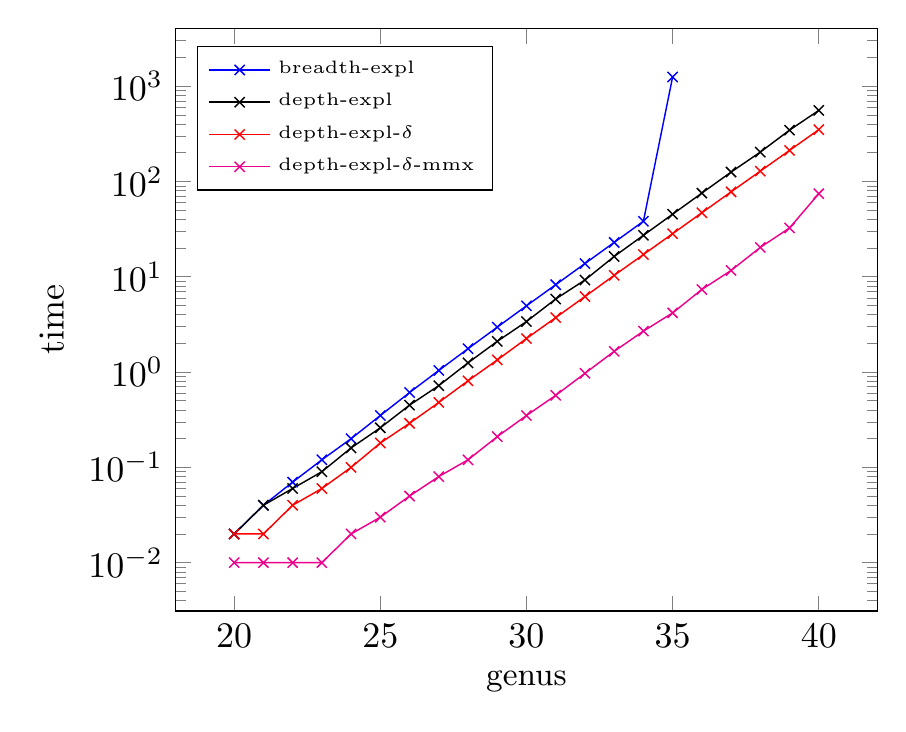
\begin{tikzpicture}[scale=1.3]
        \begin{semilogyaxis}[xlabel=\small genus,ylabel=time,legend pos=north west,legend cell align=left]
        \addplot [color=blue,mark=x] coordinates {
            (20,0.02)
            (21,0.04)
            (22,0.07)
            (23,0.12)
            (24,0.2)
            (25,0.35)
            (26,0.61)
            (27,1.04)
            (28,1.76)
            (29,2.96)
            (30,4.96)
            (31,8.26)
            (32,13.77)
            (33,22.95)
            (34,38.22)
            (35,1250.88)
        };
       \addplot [color=black,mark=x] coordinates {
			(20,0.02)	
            (21,0.04)
            (22,0.06)
            (23,0.09)
            (24,0.16)
            (25,0.26)
            (26,0.45)
            (27,0.72)
            (28,1.25)
            (29,2.1)
            (30,3.39)
            (31,5.85)
            (32,9.25)
            (33,16.34)
            (34,27.23)
            (35,45.39)
            (36,75.58)
            (37,125.59)
            (38,203.56)
            (39,346.02)
            (40,557.51)
        };
         \addplot [color=red,mark=x] coordinates {
			(20,0.02)	
            (21,0.02)
            (22,0.04)
            (23,0.06)
            (24,0.1)
            (25,0.18)
            (26,0.29)
            (27,0.48)
            (28,0.81)
            (29,1.34)
            (30,2.25)
            (31,3.73)
            (32,6.2)
            (33,10.35)
            (34,17.11)
            (35,28.35)
            (36,46.99)
            (37,77.89)
            (38,128.53)
            (39,212.1)
            (40,349.98)
        };
        \addplot [color=magenta,mark=x] coordinates {
			(20,0.01)	
            (21,0.01)
            (22,0.01)
            (23,0.01)
            (24,0.02)
            (25,0.03)
            (26,0.05)
            (27,0.08)
            (28,0.12)
            (29,0.21)
            (30,0.35)
            (31,0.57)
            (32,0.97)
            (33,1.65)
            (34,2.69)
            (35,4.18)
            (36,7.36)
            (37,11.66)
            (38,20.35)
            (39,32.55)
            (40,74.46)
        };
	%\legend style={anchor=north,at={(20,1000)}}  
        \legend{\tiny breadth-expl,\tiny depth-expl,\tiny depth-expl-$\delta$,\tiny depth-expl-$\delta$-mmx}
        \end{semilogyaxis}
    \end{tikzpicture}
    \label{F:Time:new}
    \caption{Comparison of time executions of different exploration algorithms of the tree $\mathcal{T}^{\leq g}$ on an Intel \tt{i5-3570K} CPU with $8GB$ of memory. 
The scale is logarithmic in time. 
The first version is based on a breadth-first search exploration and the peak at genus~$35$ is due to the consumption of all the memory and use of swap. 
The second version uses a depth first search exploration.
The third is based on the second one with use of decomposition numbers, it corresponds to the algorithm given in Section~\ref{S:Algo}. 
The last one is an optimisation of the third one with \MMX.}
\end{figure}



\begin{figure}[b]
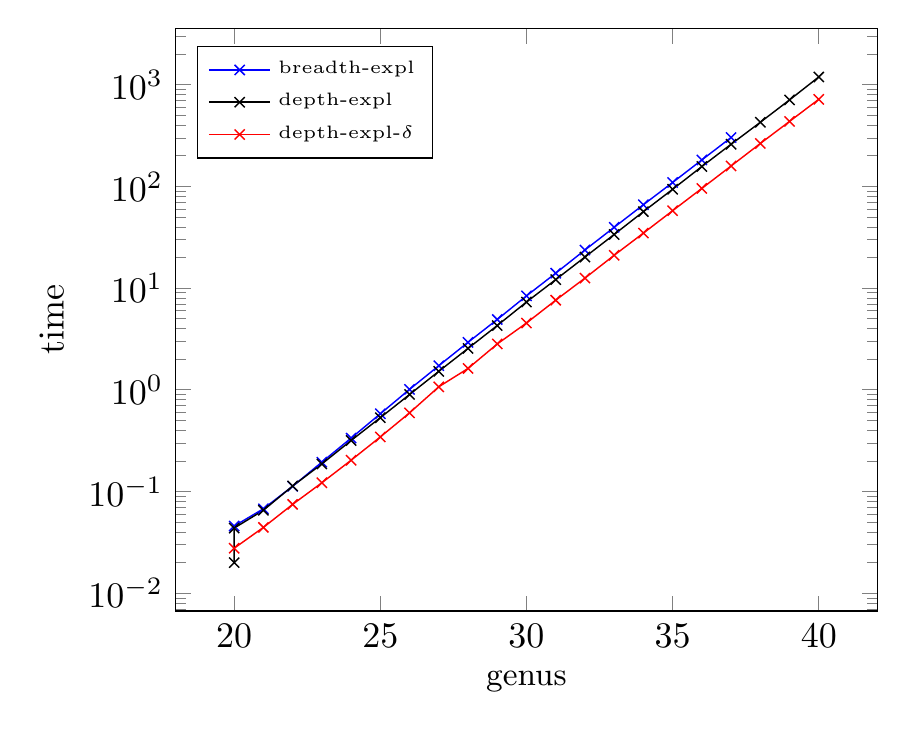
\begin{tikzpicture}[scale=1.3]
        \begin{semilogyaxis}[xlabel=\small genus,ylabel=time,legend pos=north west,legend cell align=left]
        \addplot [color=blue,mark=x] coordinates {
(20,0.045767)
(21,0.067697)
(22,0.112697)
(23,0.194646)
(24,0.335412)
(25,0.581481)
(26,1.01088)
(27,1.72613)
(28,2.9324)
(29,4.91856)
(30,8.39383)
(31,14.0308)
(32,23.7138)
(33,39.6461)
(34,66.1154)
(35,109.406)
(36,182.331)
(37,302.765)
        };
       \addplot [color=black,mark=x] coordinates {
			(20,0.02)	
(20,0.043697)
(21,0.065487)
(22,0.113301)
(23,0.186903)
(24,0.31748)
(25,0.53251)
(26,0.899982)
(27,1.5205)
(28,2.55423)
(29,4.28809)
(30,7.30236)
(31,12.1284)
(32,20.2132)
(33,33.707)
(34,56.5415)
(35,93.7614)
(36,157.09)
(37,259.997)
(38,427.497)
(39,709.564)
(40,1192.81)
        };
         \addplot [color=red,mark=x] coordinates {
(20,0.027708)
(21,0.044416)
(22,0.074789)
(23,0.122006)
(24,0.203155)
(25,0.344143)
(26,0.594073)
(27,1.07134)
(28,1.622)
(29,2.82573)
(30,4.53882)
(31,7.60975)
(32,12.5442)
(33,21.0466)
(34,34.7638)
(35,57.7621)
(36,95.6878)
(37,158.95)
(38,264.495)
(39,436.146)
(40,719.347)
        };
        \addplot [color=magenta,mark=x] coordinates {

        };
	%\legend style={anchor=north,at={(20,1000)}}  
        \legend{\tiny breadth-expl,\tiny depth-expl,\tiny depth-expl-$\delta$}
        \end{semilogyaxis}
    \end{tikzpicture}
    \label{F:Time}
    \caption{Comparison of time executions of different exploration algorithms of the tree $\mathcal{T}^{\leq g}$ on an Intel \tt{i5-3570K} CPU with $8GB$ of memory. 
The scale is logarithmic in time. 
The first version is based on a breadth-first search exploration and the peak at genus~$35$ is due to the consumption of all the memory and use of swap. 
The second version uses a depth first search exploration.
The third is based on the second one with use of decomposition numbers, it corresponds to the algorithm given in Section~\ref{S:Algo}. 
The last one is an optimisation of the third one with \MMX.}
\end{figure}


\footnotesize
\bibliographystyle{ieeetr}
\bibliography{biblio}


\end{document}


